\section{SIMULATION RESULT}

The proposed strategy is implemented and tested using the Robot Operating System (ROS) framework. In order to prove the efficiency of our decentralised strategy, we compared it with the coordinated centralised market model described in \cite{Burgard2005}. Experiments were performed in the two different indoor environments (Fig. \ref{fig:scenarios}) with two, three and five mobile robots. The start pose of the mobile robot was the same for each run. The results are presented as average of 10 runs for each set. The simulation setup is shown in the Table \ref{tab:table1}.


\begin{figure}[t]
    \setcounter{subfigure}{0}
     \begin{center}
        \subfigure[][]{\label{fig:office}
            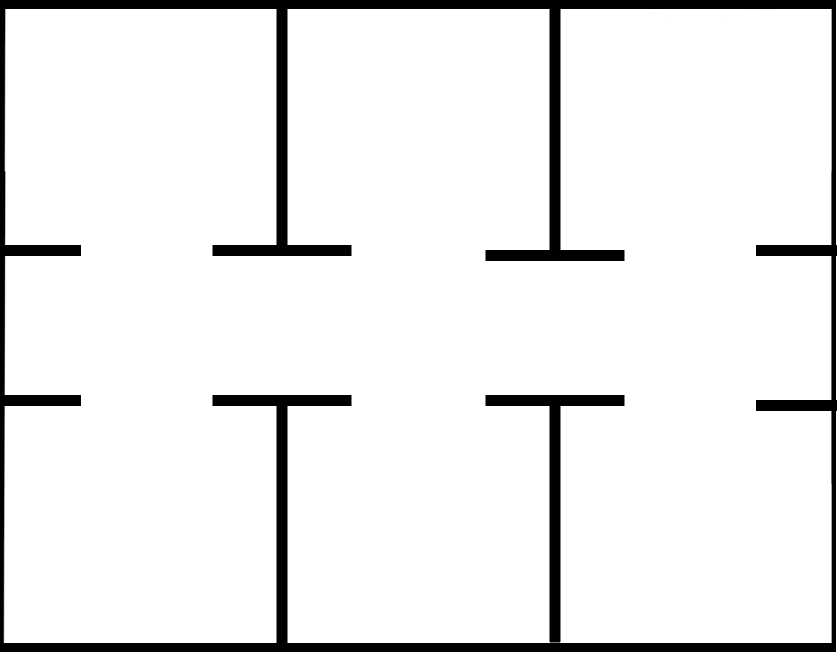
\includegraphics[width=0.47\columnwidth]{office1.png}
        }\hfill
        \subfigure[]{\label{fig:unstructured}
           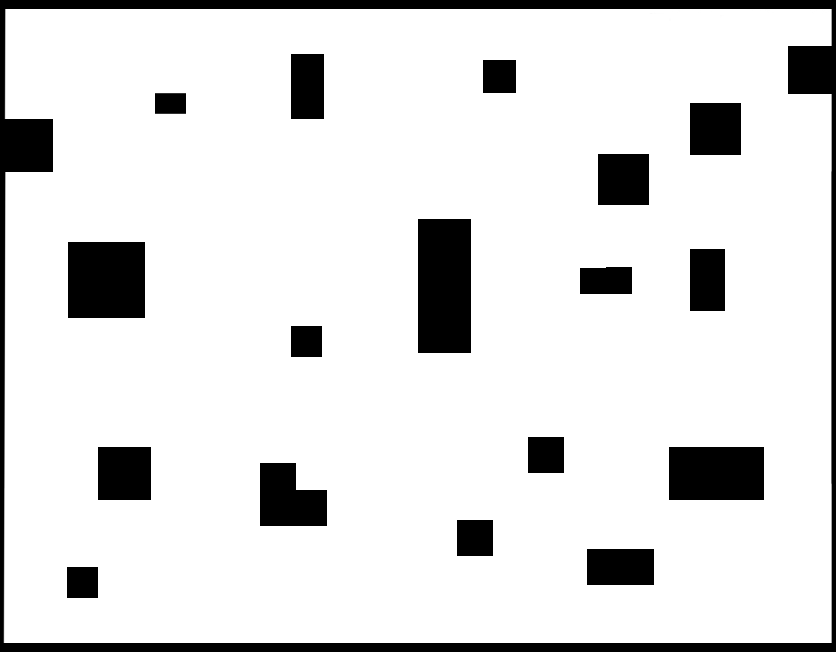
\includegraphics[width=0.47\columnwidth]{unstructured.png}}
    \end{center}
    \caption{%
       Benchmark scenarios. The terrains cover the flat surface 40 x 20 $m^{2}$ with static obstacles. \subref{fig:office} Office-like scenario; \subref{fig:unstructured} Unstructured scenario.
     }%
   \label{fig:scenarios}
\end{figure}




\begin{figure*}[h!]
     \begin{center}
     \setcounter{subfigure}{0}
%
        \subfigure[\hspace{0.1cm} Total exploration time for centralised and decentralised strategy in the office scenario for the different size of the mobile robot team]{%
            \label{fig:tt-office-a}
            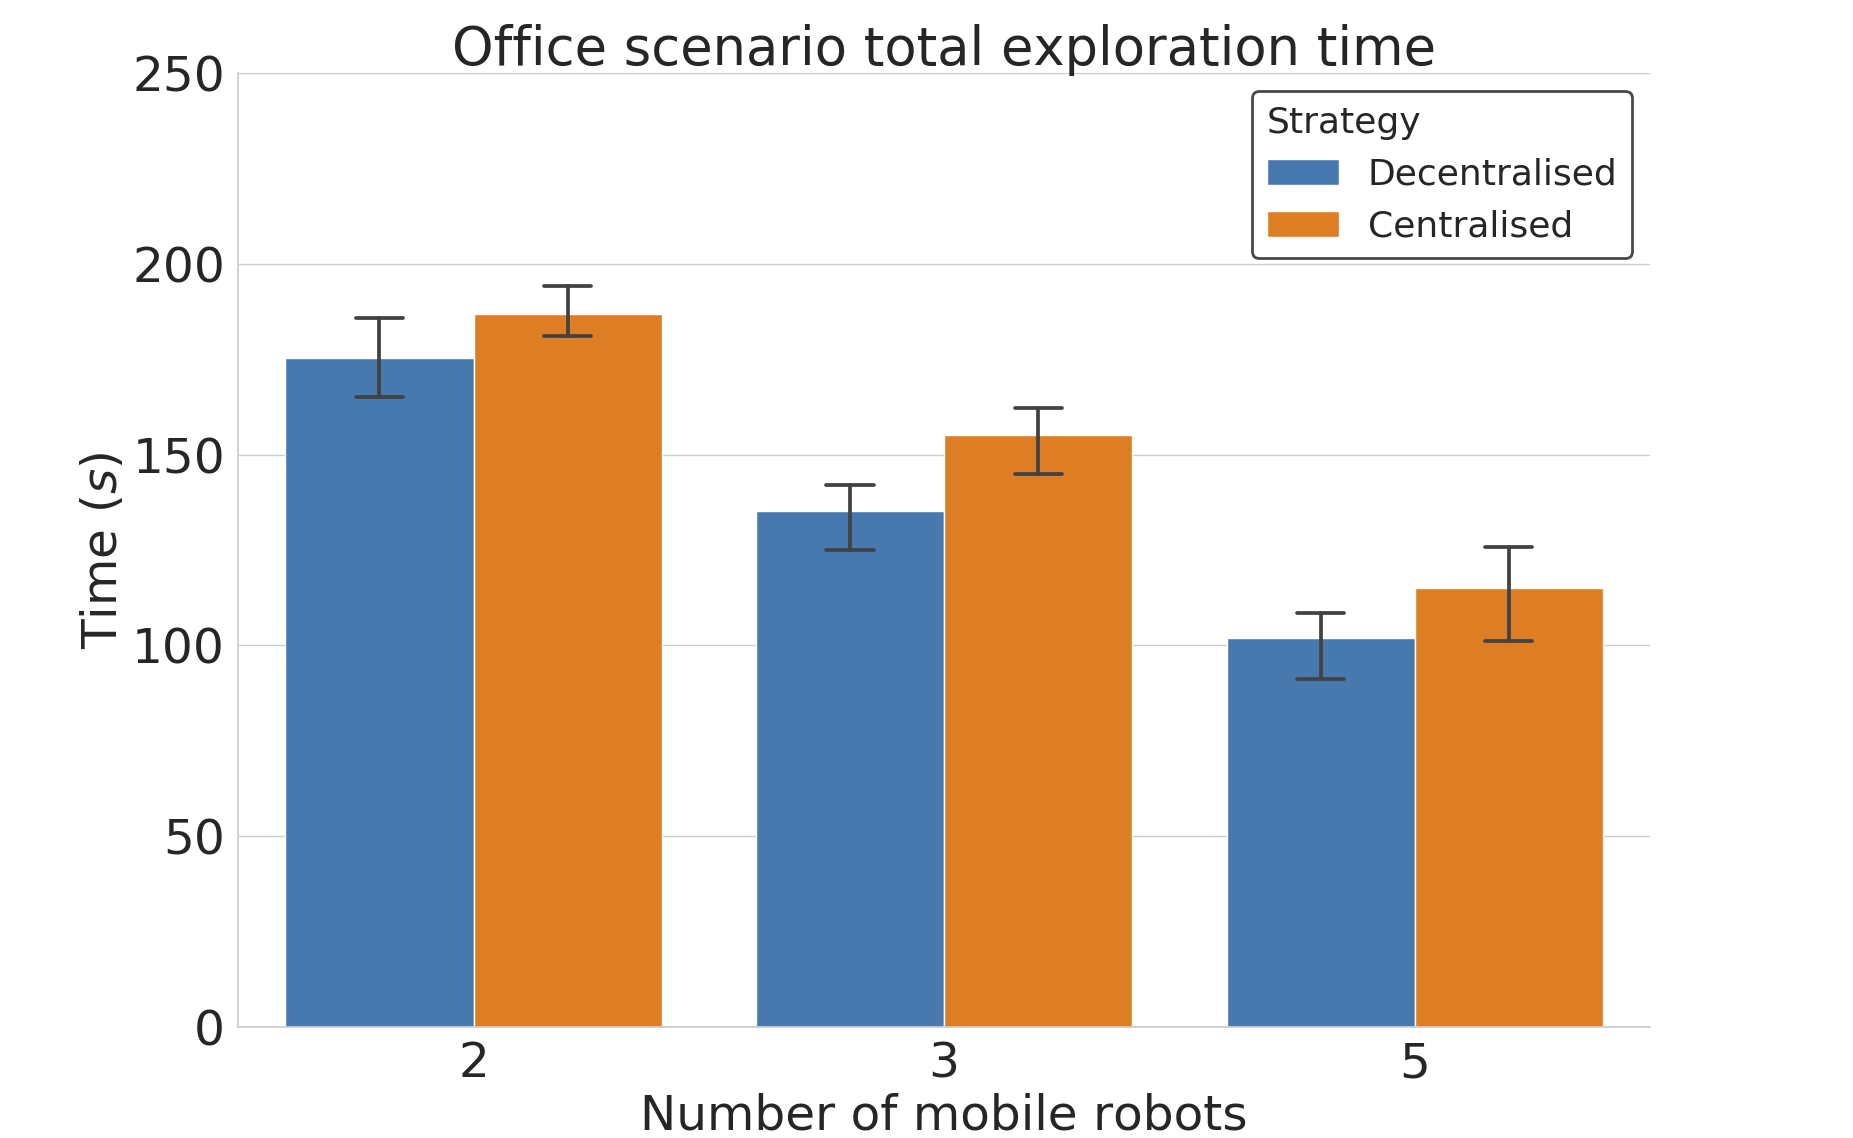
\includegraphics[width=0.46\textwidth]{office_total_e_time.png}
        }\hfill
        \subfigure[\hspace{0.1cm} Total exploration time for centralised and decentralised strategy in the unstructured scenario for the different size of the mobile robot team]{%
           \label{fig:tt-unstructired-b}
           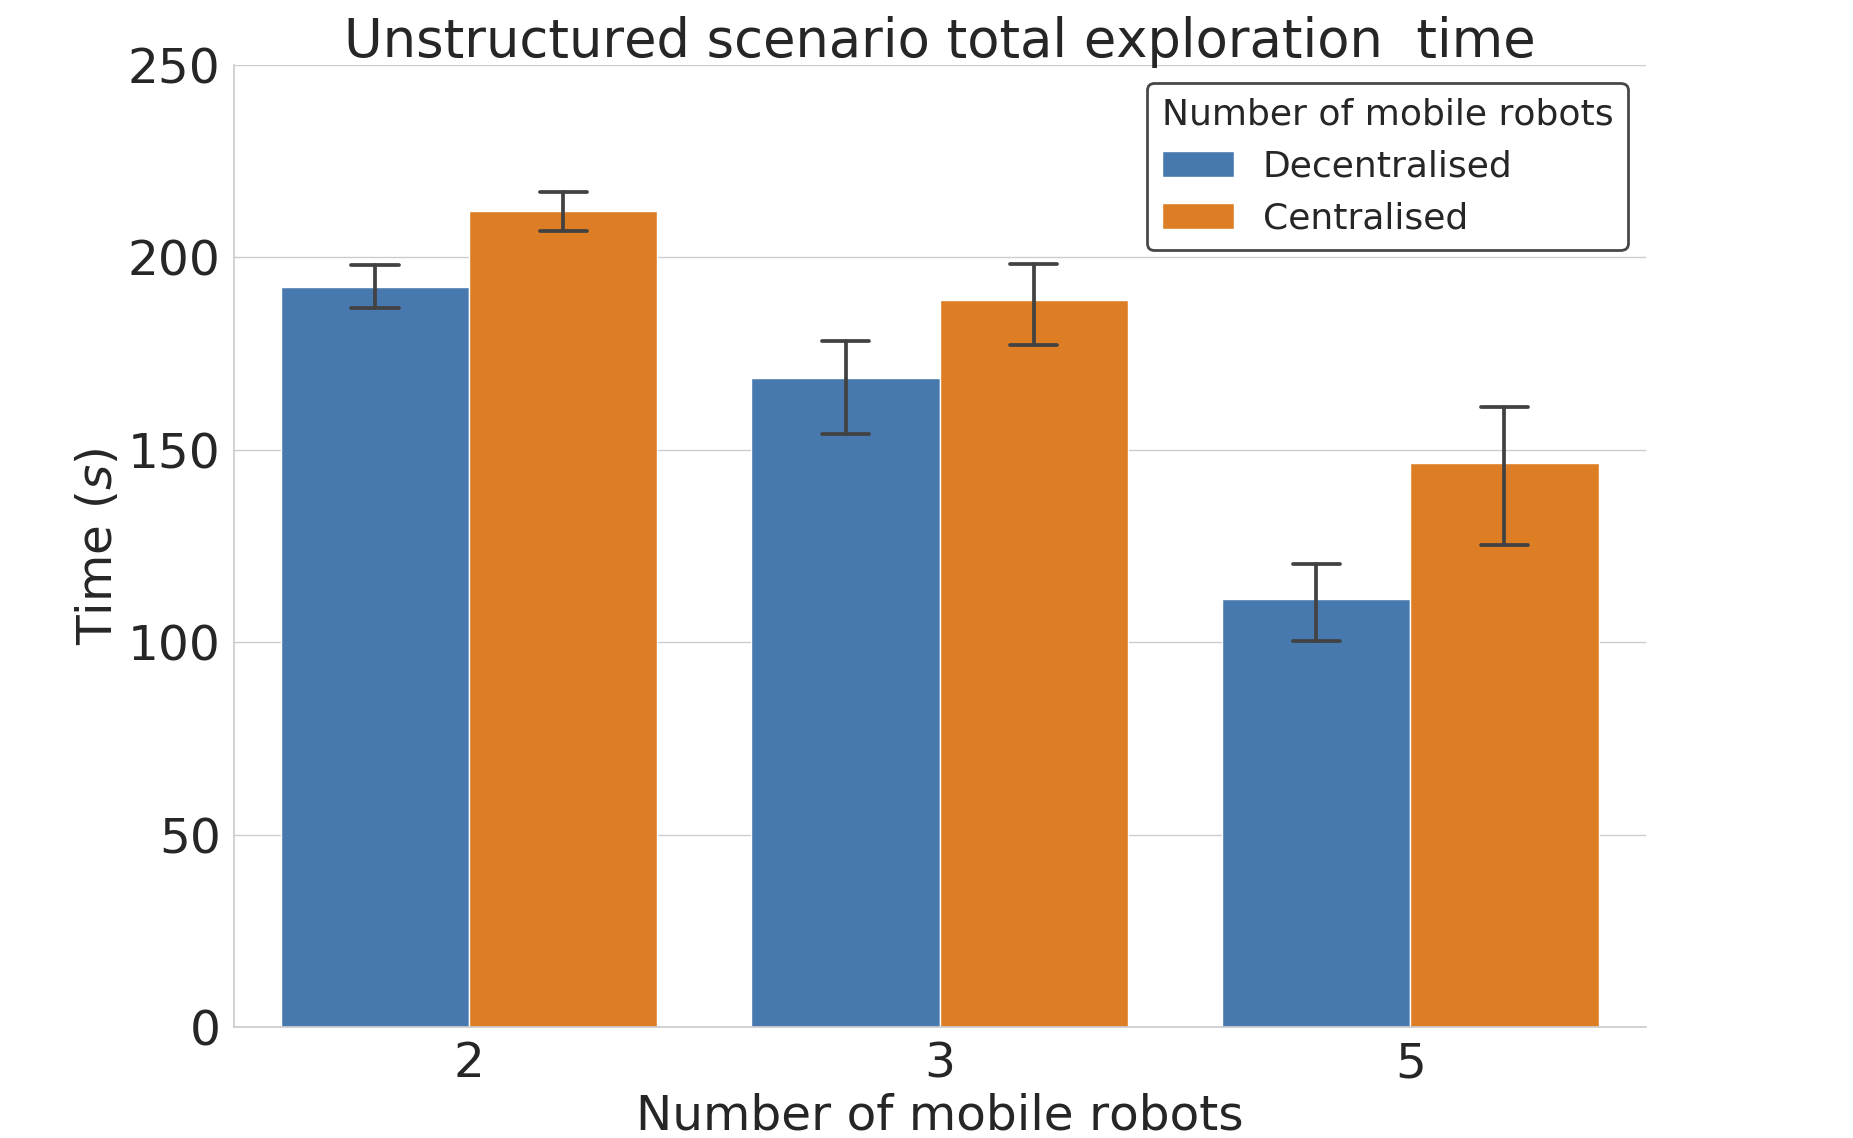
\includegraphics[width=0.46\textwidth]{unstructured_total_e_time.png}
        }\\ %  ------- End of the first row ----------------------%
        \subfigure[\hspace{0.1cm} Average path length per robot for centralised and decentralised strategy in the office scenario for the different size of the mobile robot team]{%
            \label{fig:path-office-c}
            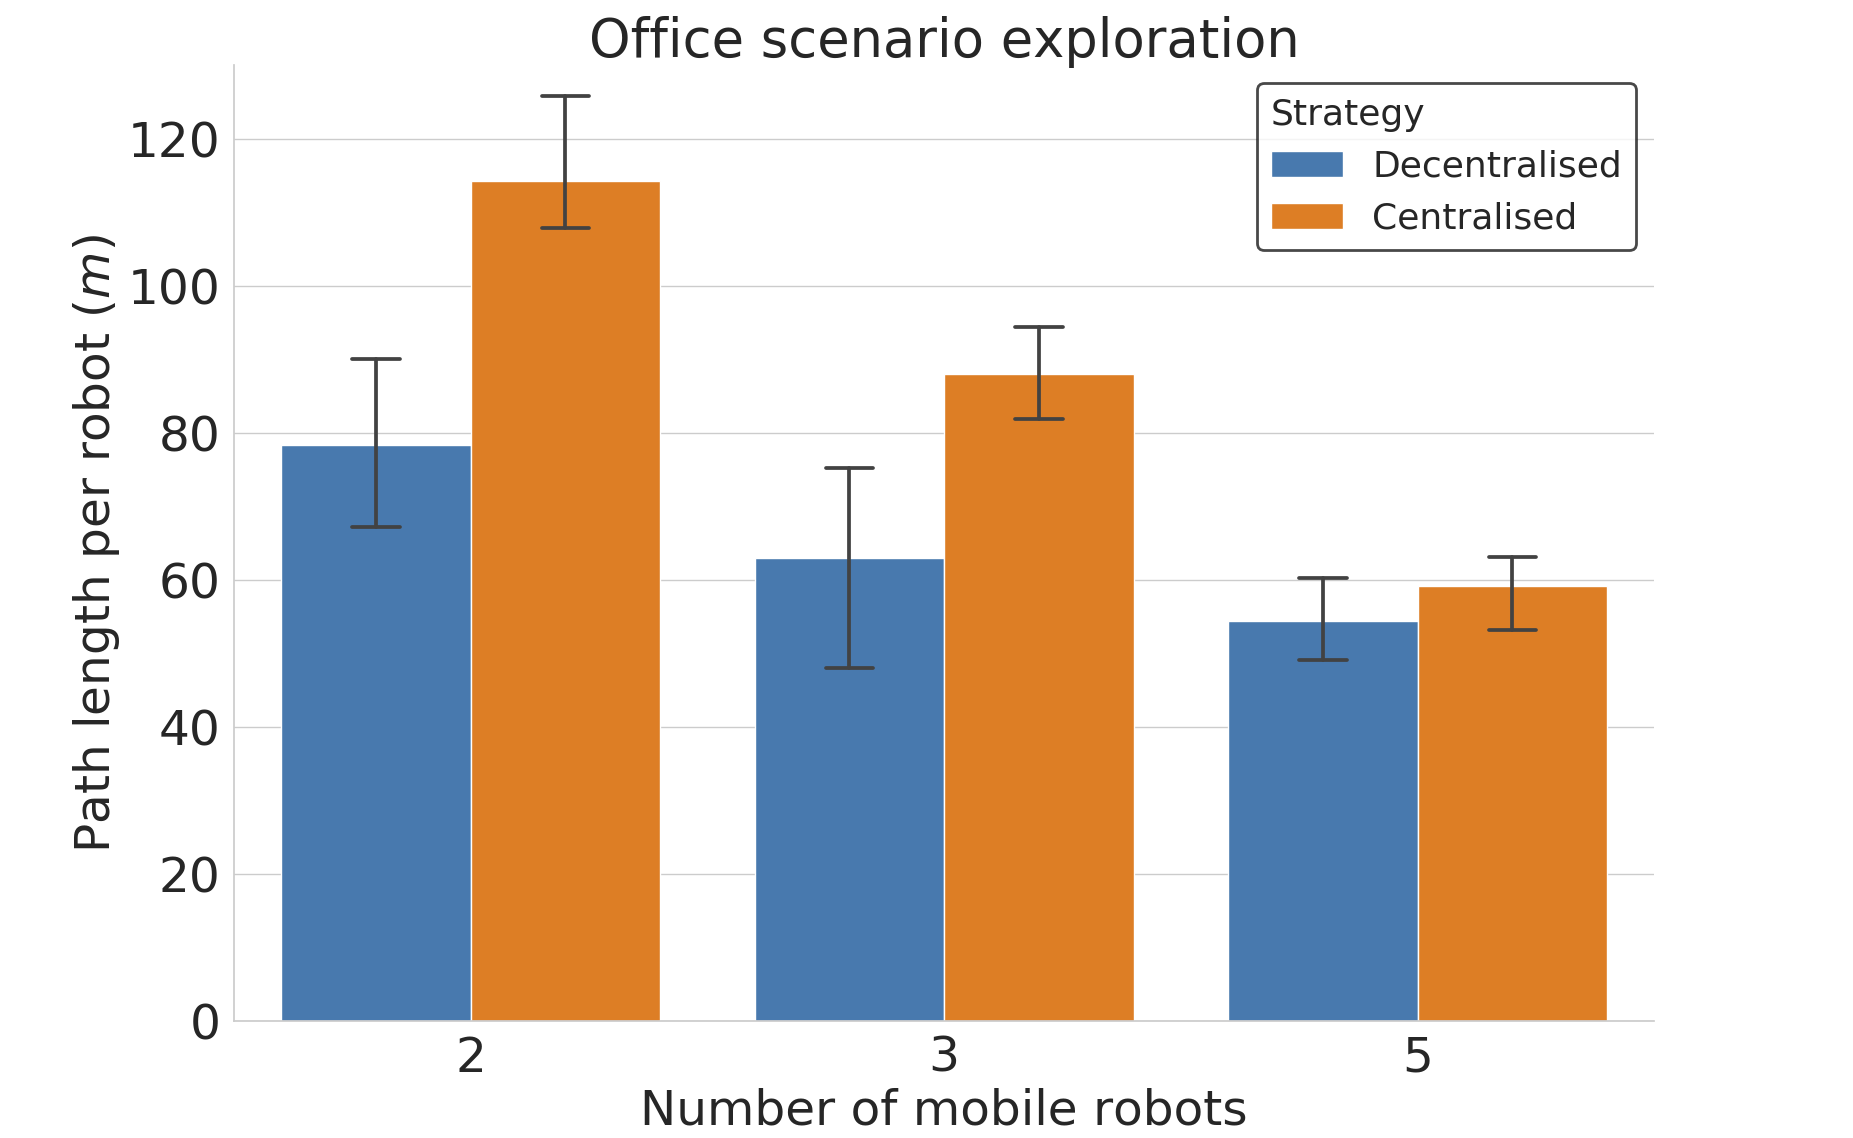
\includegraphics[width=0.46\textwidth]{office_path_length_per_robot.png}
        }\hfill
        \subfigure[\hspace{0.1cm} Average path length per robot for centralised and decentralised strategy in the unstructured scenario for the different size of the mobile robot team]{%
            \label{fig:path-unstructured-d}
            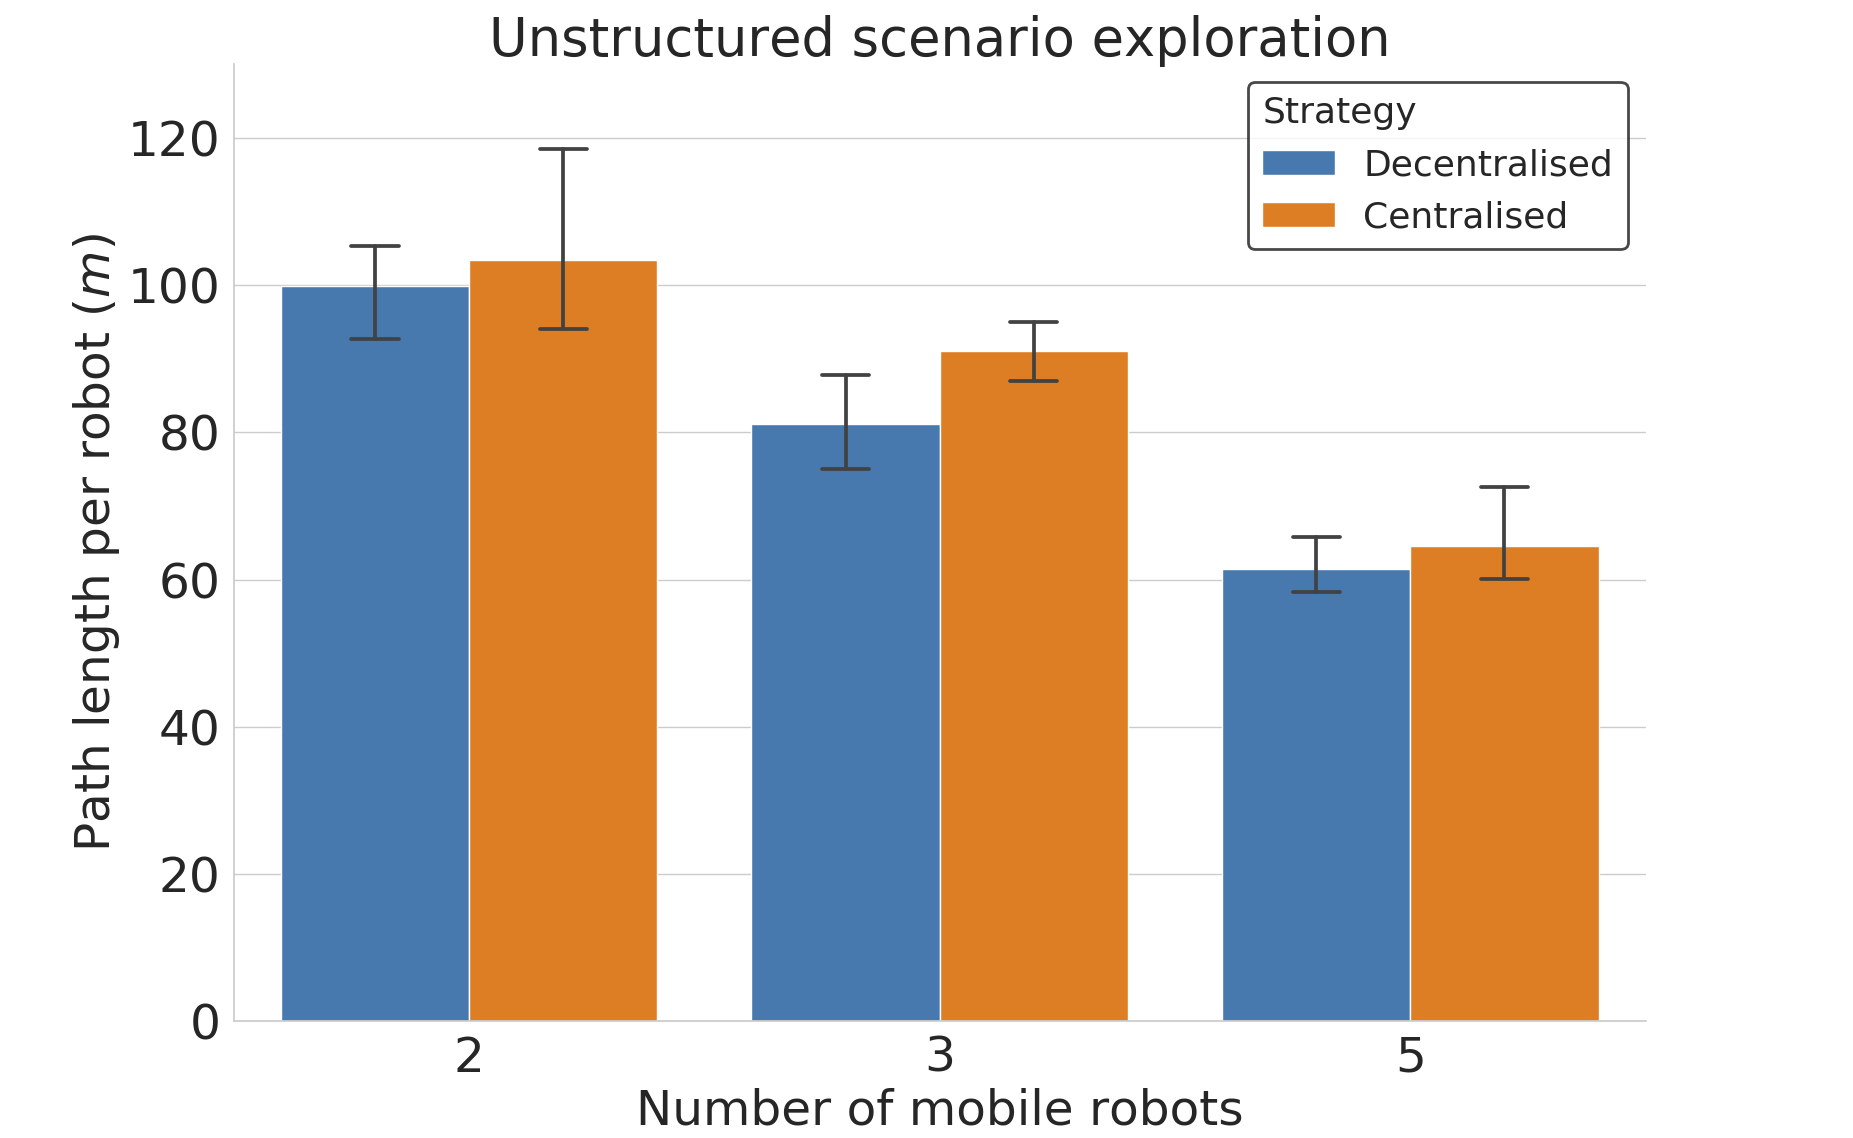
\includegraphics[width=0.46\textwidth]{unstructured_path_lenght_per_robot.png}
        }%
%
    \end{center}
    \caption{%
       The comparison of the centralised and decentralised strategy for office and unstructured scenarios in the term of total exploration time \subref{fig:tt-office-a}, \subref{fig:tt-unstructired-b} and in the term of path length per robot \subref{fig:path-office-c}, \subref{fig:path-unstructured-d}.
     }%
   \label{fig:time_and_path_subfigures}
\end{figure*}

\begin{table}[t]
  \centering
    \caption{Simulation setup.}
    \label{tab:table1}
    \begin{tabular}{ll} 
\hline
\rule{0pt}{2.2ex}
\textbf{Mobile robot features} &  \\ 
\quad Model & Pioneer P3-DX  \\
\quad Maximum speed & 1.5 (m/s) \\
\quad Laser range & 10 (m) \\
\quad Laser scan window & 250 ($^{\circ}$) \\
\hline
\rule{0pt}{2.2ex}
\textbf{Environment features}  \\ 
\quad Terrain & 40 x 20 ({m}^2) \\
\quad Wall height & 0.5 (m) \\
\quad Initial mobile robot position & Center \\
\hline
\rule{0pt}{2.2ex}
\textbf{Decentralised strategy parameters} & \\
\quad  \lambda_{u} & 0.9\\
\quad \lambda_{f} & 1.2\\
\quad $r$ & 1.0\\
\quad $r_{f}$ & 3.0\\
\hline
\rule{0pt}{2.2ex}
%\quad Intel Core i7-8550U @ 1.80GHz & \\
\end{tabular}
\end{table}

The comparison of the centralised strategy and our decentralised strategy is shown in Fig. \ref{fig:coverage_subfigures} and Fig. \ref{fig:time_and_path_subfigures} using the indicators defined as follows:

\textbf{Coverage Ratio (CR)}: percentage of the accessible terrain covered by the team. Calculated as:  \( \frac{\text{explored cells} \cdot 100}{\text{accessible cells}} \).

\textbf{Path Length (PL)}: distance travelled by a mobile robot measured in meters.

\textbf{Total exploration Time (TT)}: time elapsed from the beginning until the end of exploration measured in seconds.\\

First of all, it is interesting to see how the coverage evolves over time. Fig. \ref{fig:coverage_subfigures} shows \textbf{CR} over time for both centralised and decentralised multi-robot exploration strategies in the office scenario as well as in the unstructured scenario. We report the time it takes to cover 50, 75, 90 and 99 percent of the environment. Obviously, it takes almost the same time to explore a few last cells and 25 percent (from 75 to 90 percent) of the environment. In the both scenarios, the decentralised strategy needed less time to explore the same percentage of the environment. Furthermore, increase in performance was greater for larger number of mobile robots. For instance, using decentralised strategy, it took 14 percent less time for three mobile robots to explore unstructured environment compared to centralised strategy, and for five mobile robots the increase was 25 percent.  

When we compare the \textbf{TT} for the both strategies (Fig. \ref{fig:time_and_path_subfigures} \subref{fig:tt-office-a} and \subref{fig:tt-unstructired-b}), it shows that five mobile robots perform better than two and three, while there is a small difference in having three robots instead of two. The decentralised strategy performs faster than the centralised strategy.

The next parameter of interest for comparison is \textbf{PL} shown in the Fig. \ref{fig:time_and_path_subfigures} \subref{fig:path-office-c} and \subref{fig:path-unstructured-d}. We compared the average path length per robot for the different sizes of the mobile robot team for both strategies. The average path length per robot in the centralised strategy based on \cite{Burgard2005} is significantly higher compared to the proposed decentralised strategy, especially in the office scenario for two and three mobile robots. 
